%%%% CAPÍTULO 4 - RESULTADOS E DISCUSSÃO

\chapter{Desenvolvimento}\label{cap:desenvolvimento}

Este capítulo descreve como ocorreu o processo de desenvolvimento deste trabalho, esmiuçando os algoritmos, as interfaces e os processos internos de comunicação que orquestram a interação entre partes envolvidas. Além disso, esse capítulo irá demostrar o processo de adaptação e integração de um projeto existente ao PRISM para que o mesmo seja validado através da realização de uma coleta de dados, que serão usados para testar o funcionamento do processo de compartilhamento de dados entre NPIs.

\section{Visão Geral}\label{sec:desenvolvimentoVisaoGeral}

Para testar a hipótese de interoperabilidade através da troca de dados estruturados entre dois NPIs, propõe-se a simulação de uma estrutura institucional descrita pela Figura \ref{fig:estruturaSimulada}. Uma universidade que possui um projeto de pesquisa integrado com o padrão do PRISM compartilhando dados para um novo NPI. Para simplificar o diagrama, ligações tracejadas vermelhas foram usadas para simbolizar comunicação construida sobre o PRISM Middleware.

\begin{figure}[htpb]%% Ambiente figure
    \captionsetup{width=1\textwidth}
    \caption{Estrutura institucional simulada para validação do PRISM.}%% Legenda
    \label{fig:estruturaSimulada}%% Rótulo
    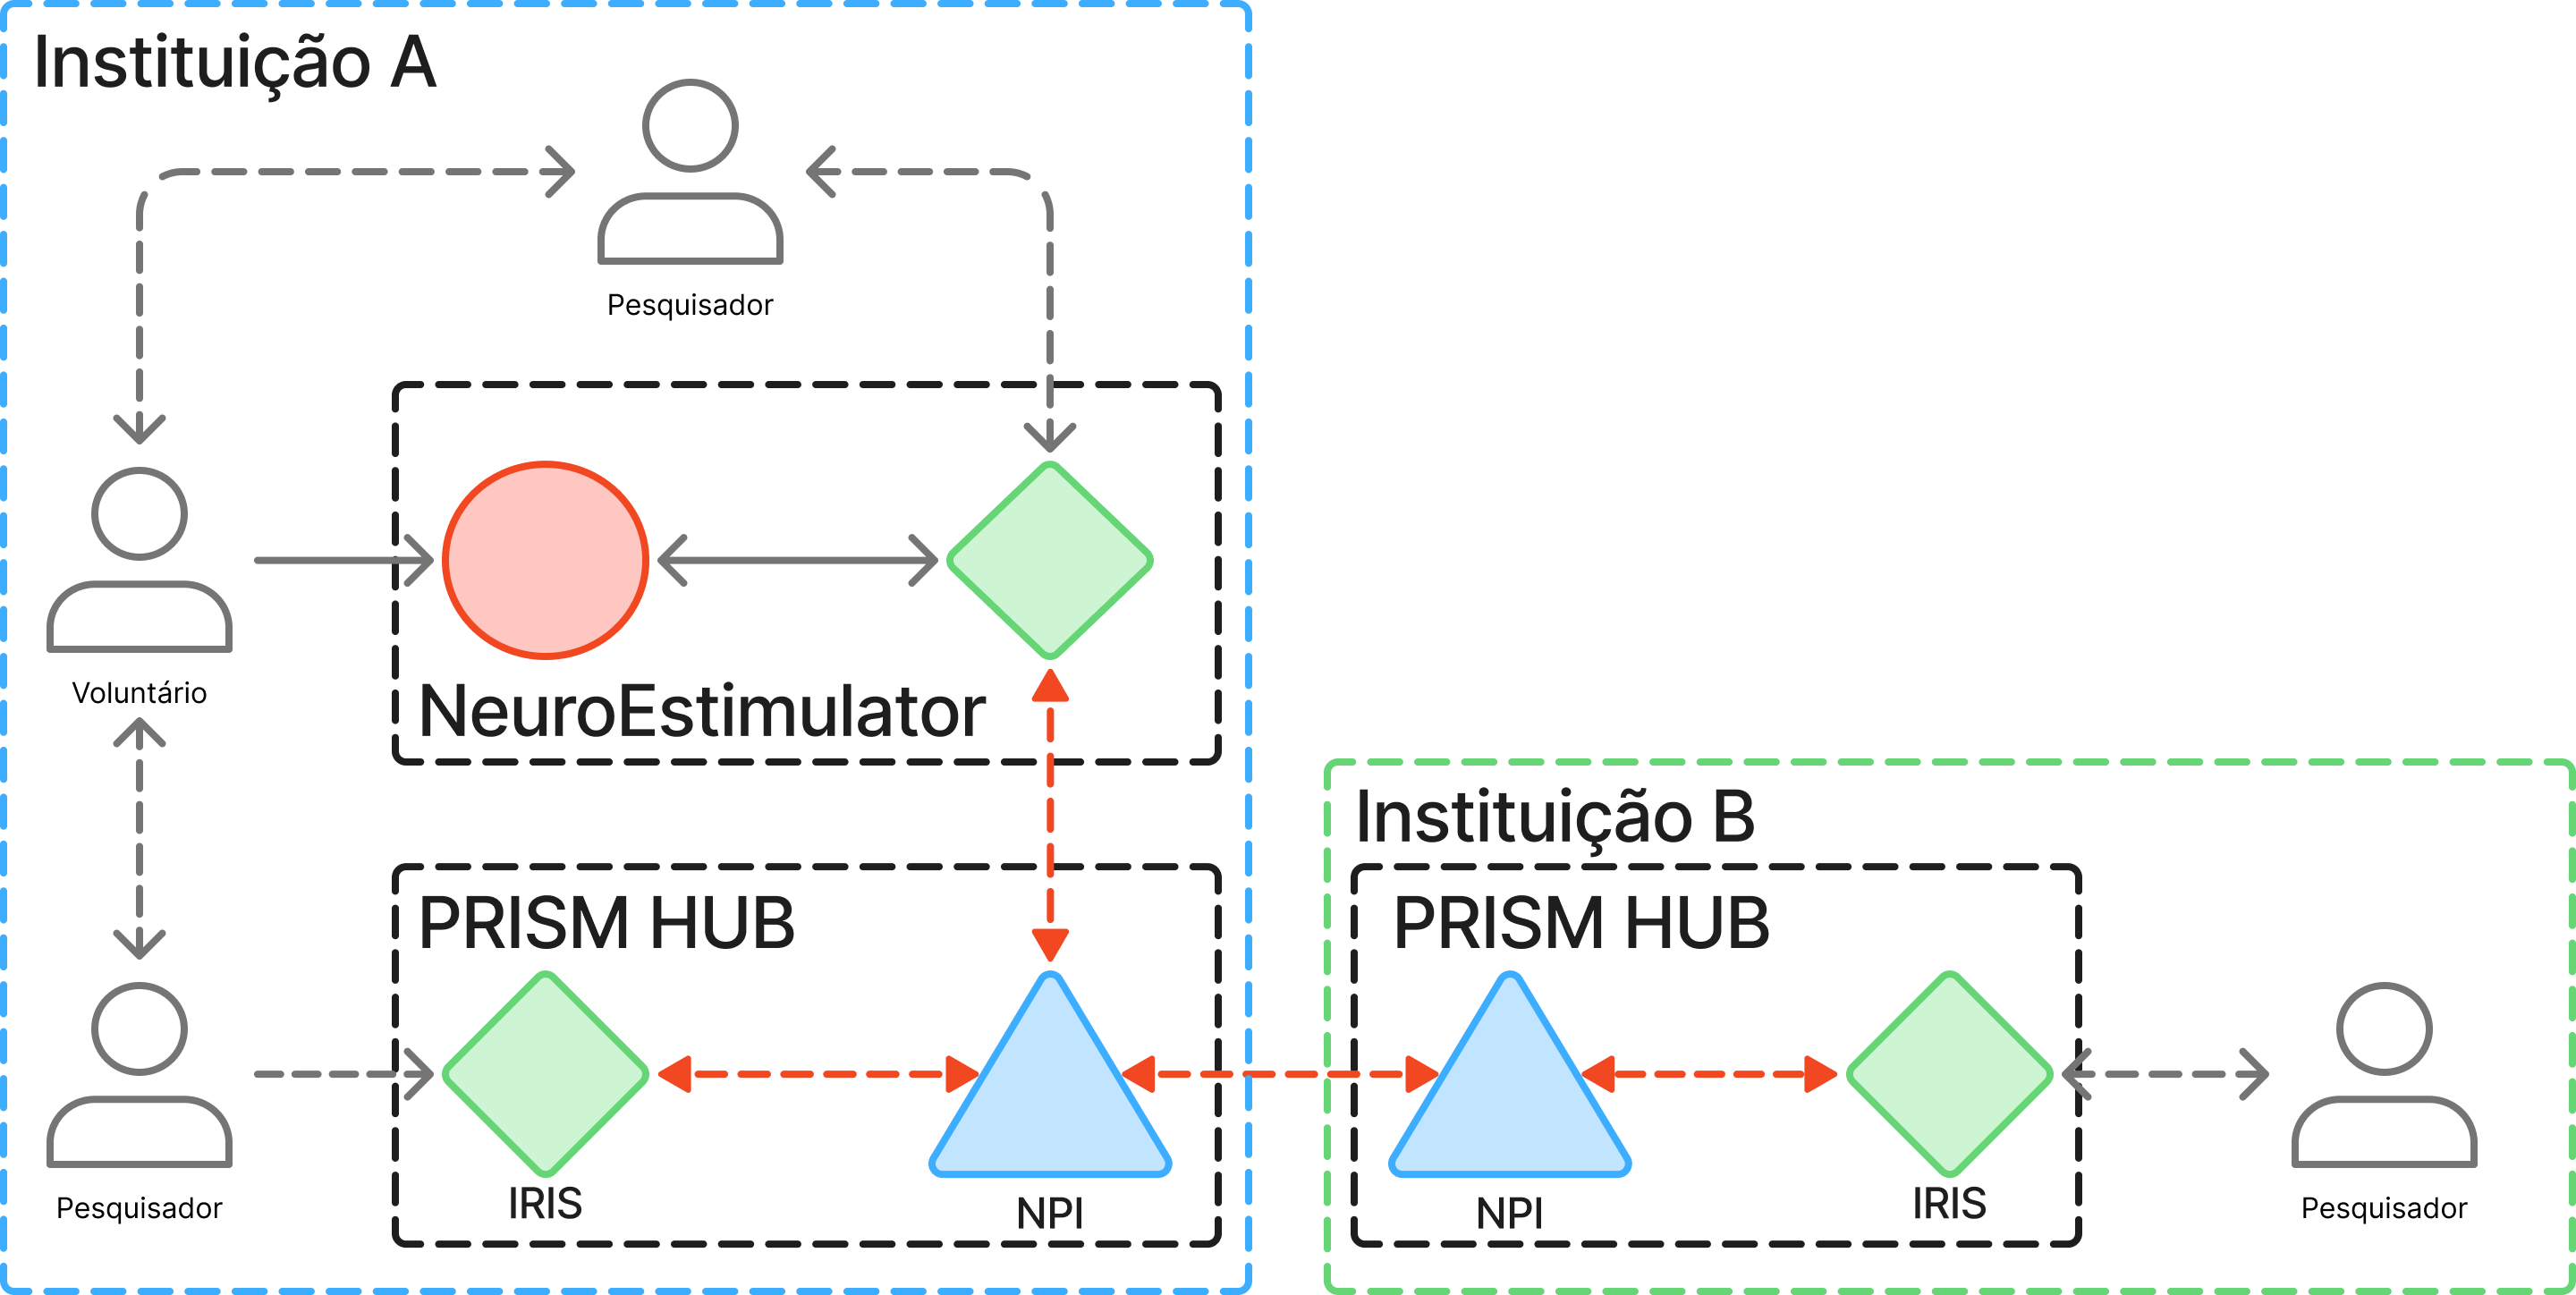
\includegraphics[scale=0.12]{figuras/Desenvolvimento/visaoGeral/estrutura-simulada.png}%% Dimensões e localização
    \fonte{Autoria própria (2026)}%% Fonte
\end{figure}

Dentro desse cenário, este trabalho estrutura o fluxo de consumo dos dados de pesquisa de uma instituição por outra. As fontes de dado e as principais comunicações previstas pelo modelo são apresentadas na Figura \ref{fig:fluxo-simulado}, na qual pesquisadores criam e utilizam rótulos para adicionar contexto aos biossinais obtidos durante as coletas.

\begin{figure}[htpb]%% Ambiente figure
\captionsetup{width=1\textwidth}
\caption{Fluxo de dados pretendido entre as instituições simuladas.}%% Legenda
\label{fig:fluxo-simulado}%% Rótulo
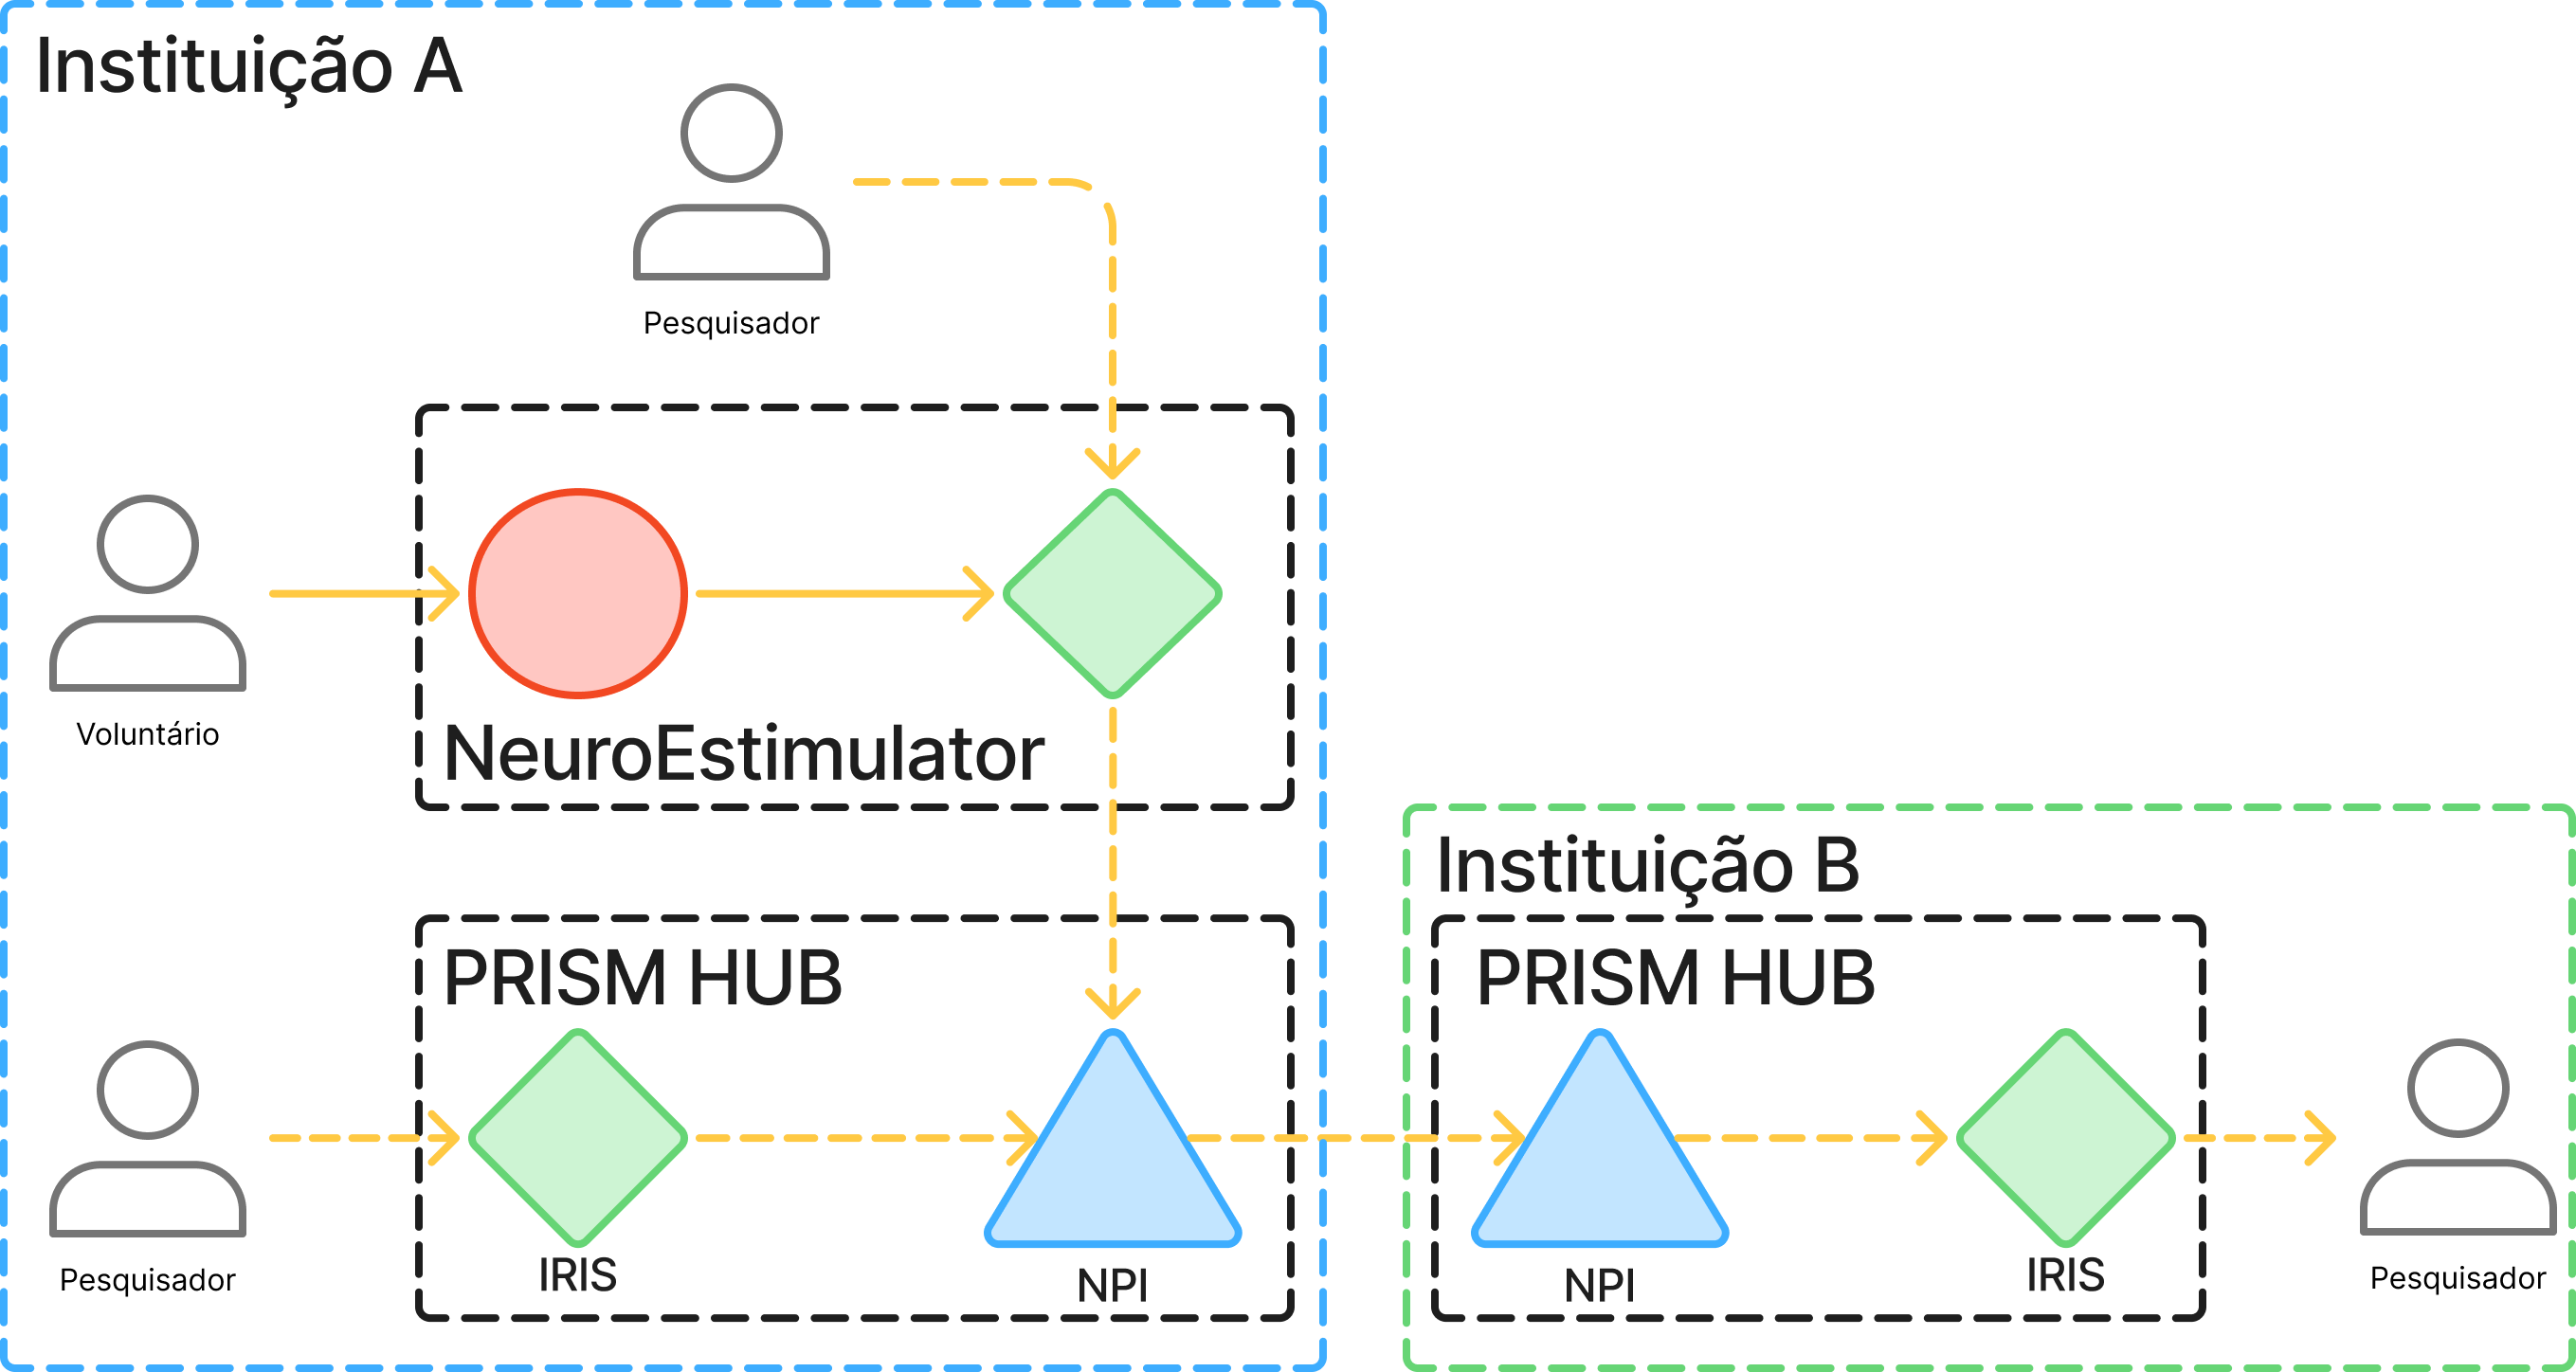
\includegraphics[scale=0.12]{figuras/Desenvolvimento/visaoGeral/fluxo-simulado.png}%% Dimensões e localização
\fonte{Autoria própria (2026)}%% Fonte
\end{figure}

A materialização desse cenário exigiu o desenvolvimento de quatro artefatos, cada um responsável por validar uma característica específica do padrão. O \textbf{NPI} é a API que serve de base à infraestrutura de interoperabilidade e aplica as regras de identificação e autenticação definidas pelo PRISM, sendo responsável por provar a viabilidade da camada de \textit{middleware}. O \textbf{IRIS} é a interface gráfica web que permite ao usuário operar o NPI e configurar suas conexões e dados, evidenciando a integração de aplicações generalistas ao padrão. O \textbf{IRIS Mobile} é a aplicação móvel que substitui a interface anteriormente utilizada pelo NeuroEstimulator, demonstrando que clientes em plataformas heterogêneas consomem o mesmo contrato do NPI. Por fim, o firmware do \textbf{NeuroEstimulator} foi refatorado para fornecer aumentar a taxa de amostragem e expor um fluxo contínuo de biossinal sobre o protocolo Bluetooth do dispositivo, ilustrando a adaptabilidade de dispositivos legados ao padrão.

A delimitação acima resulta das restrições de equipe (um único autor) e de prazo (ciclo acadêmico de um ano) aplicadas ao trabalho. Nessas condições, priorizou-se a profundidade do NPI — componente central da hipótese — em detrimento da amplitude do padrão: optou-se por uma única modalidade de biossinal (sEMG), um único projeto-exemplo e federação entre apenas dois nós. Essas escolhas preservam a capacidade do experimento de testar a hipótese, uma vez que o contrato do NPI foi implementado de forma agnóstica ao tipo de biossinal, mantendo o padrão extensível a outras modalidades sem alteração da camada de \textit{middleware}.

O restante deste capítulo detalha cada um dos artefatos apresentados nesta visão geral, na ordem em que se conectam ao fluxo de dados ilustrado na Figura \ref{fig:fluxo-simulado}. A Seção \ref{sec:DesenvolvimentoNPI} descreve a arquitetura interna do Nó de Pesquisa Interoperável, com ênfase na camada de \textit{PRISM Middleware} responsável pelas rotinas de identificação, autenticação e troca segura entre nós. A Seção \ref{sec:desenvolvimentoIRIS} apresenta o IRIS, a interface web generalista que opera sobre o NPI e materializa o papel de aplicação no modelo PRISM. A Seção \ref{sec:desenvolvimentoIRISMobile} estende essa discussão para a versão móvel do IRIS, especializada na captura de biossinais e no comando do dispositivo. Por fim, a Seção \ref{sec:adaptacaoNeuroEstimulator} documenta as modificações aplicadas ao firmware do NeuroEstimulator que viabilizaram sua integração ao ecossistema, demonstrando o caminho de adaptação de dispositivos legados ao padrão.


\section{Nó de Pesquisa Interoperável}\label{sec:DesenvolvimentoNPI}

A figura \ref{fig:NPIArquitetura} mostra como é organizado o NPI internamente, a camada de middleware do PRISM envelopa todas as requisições recebidas e devolvidas pela camada de controller do nó. A camada de serviço é responsável por armazenar as regras de negócio relacionadas a armazenamento e busca das informações dentro do NPI. Os repositórios são as camadas de abstração responsáveis pela implementação das operações busca e persistência nos bancos de dados e arquivos da aplicação. Para modelagem do banco relacional foi utilizado a técnica de mapeamento de objetos relacionais (\textit{Object-Relational Mapping} — ORM) \cite{ColleyORM} através da implementação da biblioteca \textit{Entity Framework}.

\begin{figure}[htpb]%% Ambiente figure
\captionsetup{width=0.43\textwidth}
\caption{Arquitetura do NPI}%% Legenda
\label{fig:NPIArquitetura}%% Rótulo
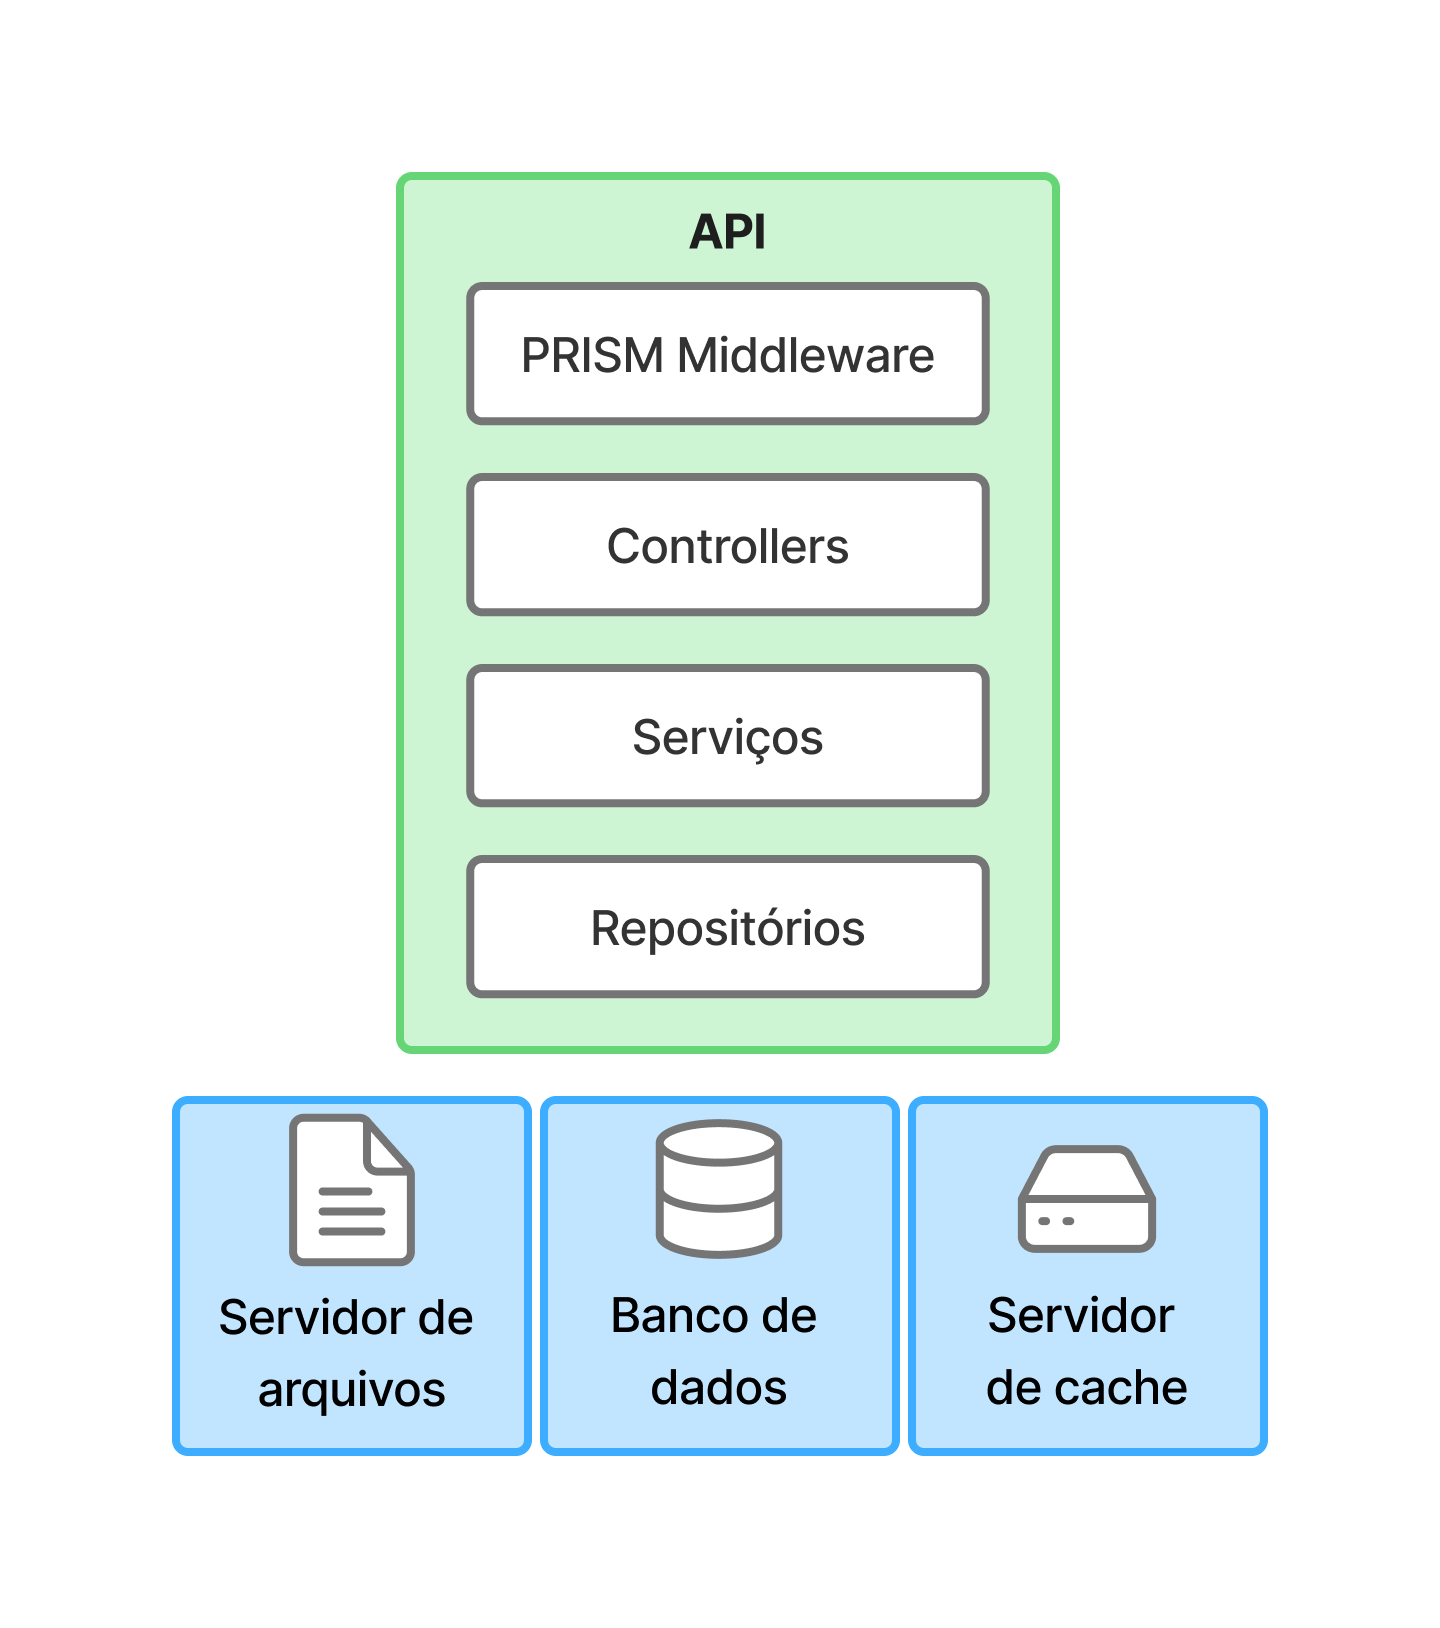
\includegraphics[scale=0.3]{figuras/Desenvolvimento/NPI/ArquiteturaNPI.png}%% Dimensões e localização
\fonte{}%% Fonte
\end{figure}

\subsection{PRISM Middleware}

O processo de criação de canal seguro, registro e identificação do solicitante é mediado pelo middleware em dois níveis, aplicação e usuário. O nível de aplicação permite que um NPI ou outra aplicação cliente de um NPI possa se registrar e autenticar de forma segura sem a intervenção de um usuário para rotinas de sincronização de dados entre nó, uma vez que o administrador do NPI autorize a aplicação cliente. Esse envelopamento garante que a troca de informações entre cliente e servidor serão criptografadas visando dificultar o roubo de informações sensíveis, mesmo em redes insegura. As figuras \ref{fig:auth-fase-1}, \ref{fig:auth-fase-2} e \ref{fig:auth-fase-3} mostram as fases do processo de inicialização da conexão com um NPI.

\begin{figure}[htpb]%% Ambiente figure
\captionsetup{width=0.43\textwidth}
\caption{Abertura de canal criptografado}%% Legenda
\label{fig:auth-fase-1}%% Rótulo
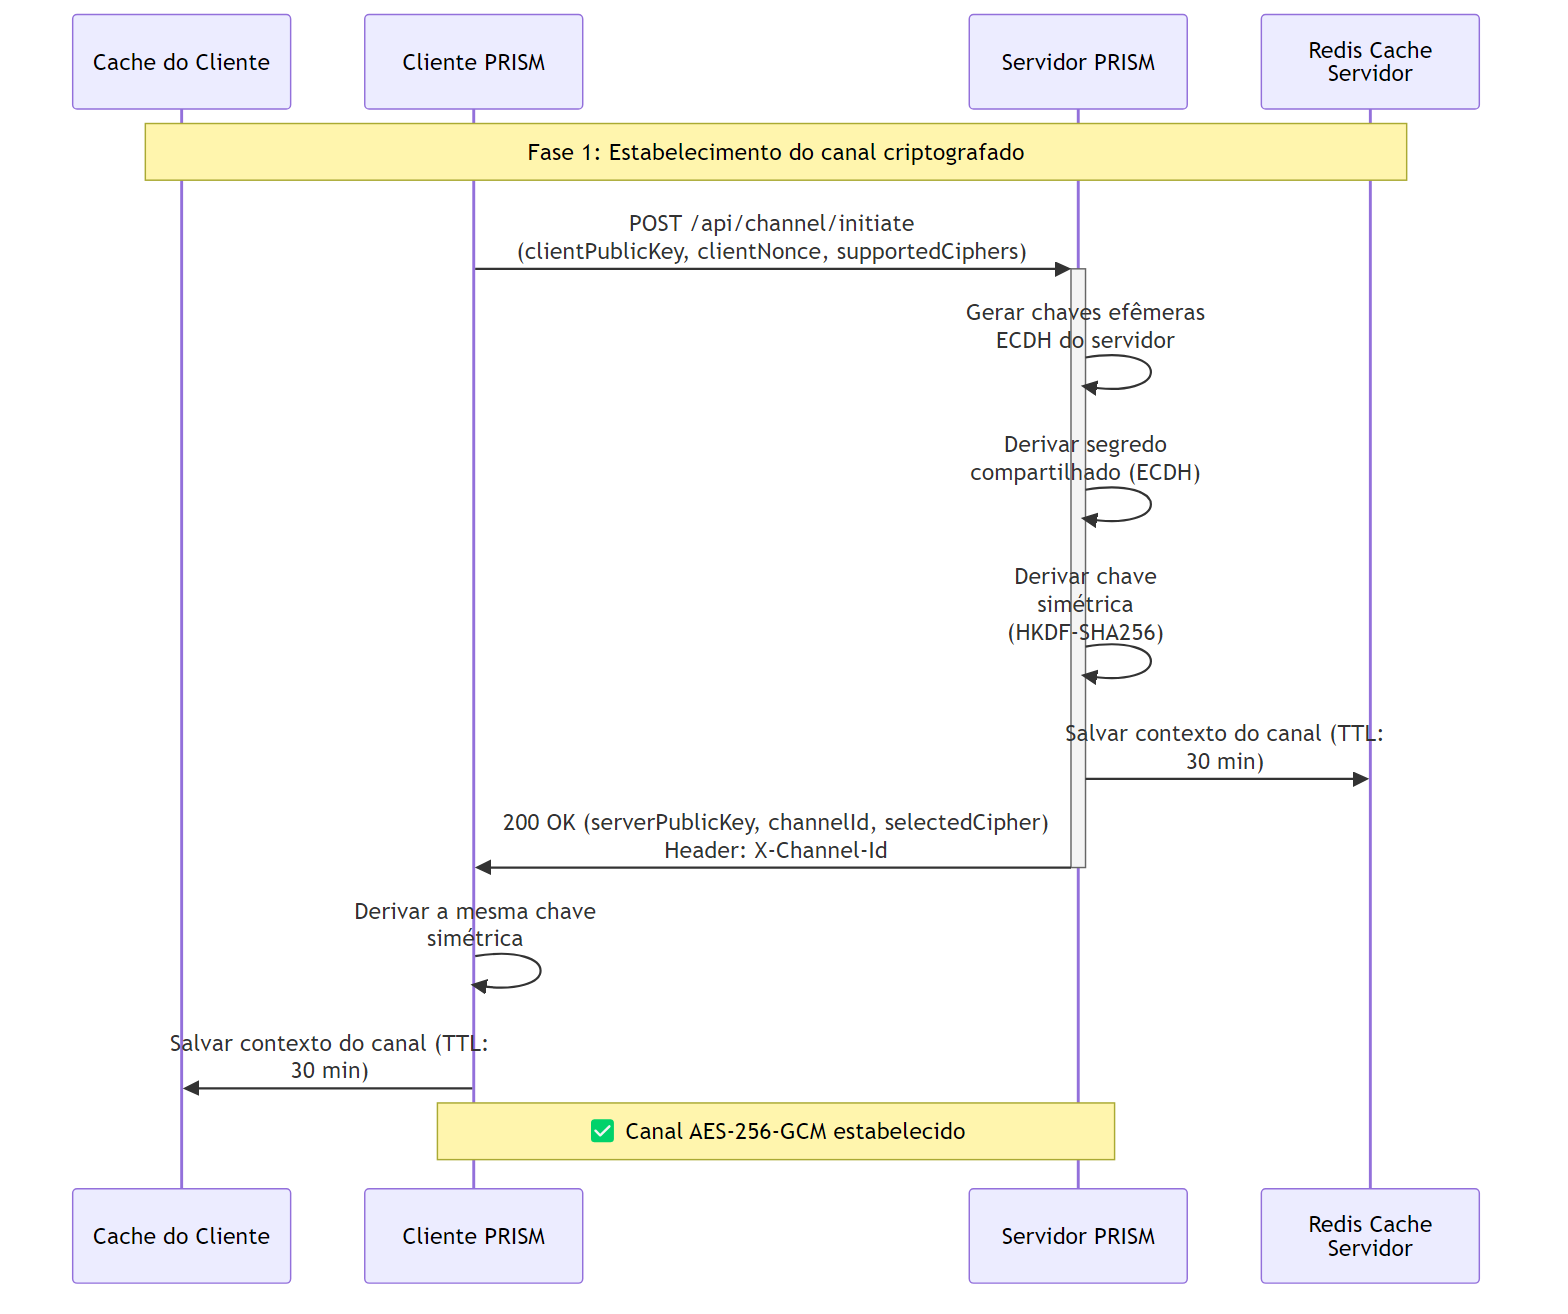
\includegraphics[scale=0.35]{figuras/Desenvolvimento/auth/fase-1.png}%% Dimensões e localização
\fonte{}%% Fonte
\end{figure}

\begin{figure}[htpb]%% Ambiente figure
\captionsetup{width=0.43\textwidth}
\caption{Registro e identificação do nó}%% Legenda
\label{fig:auth-fase-2}%% Rótulo
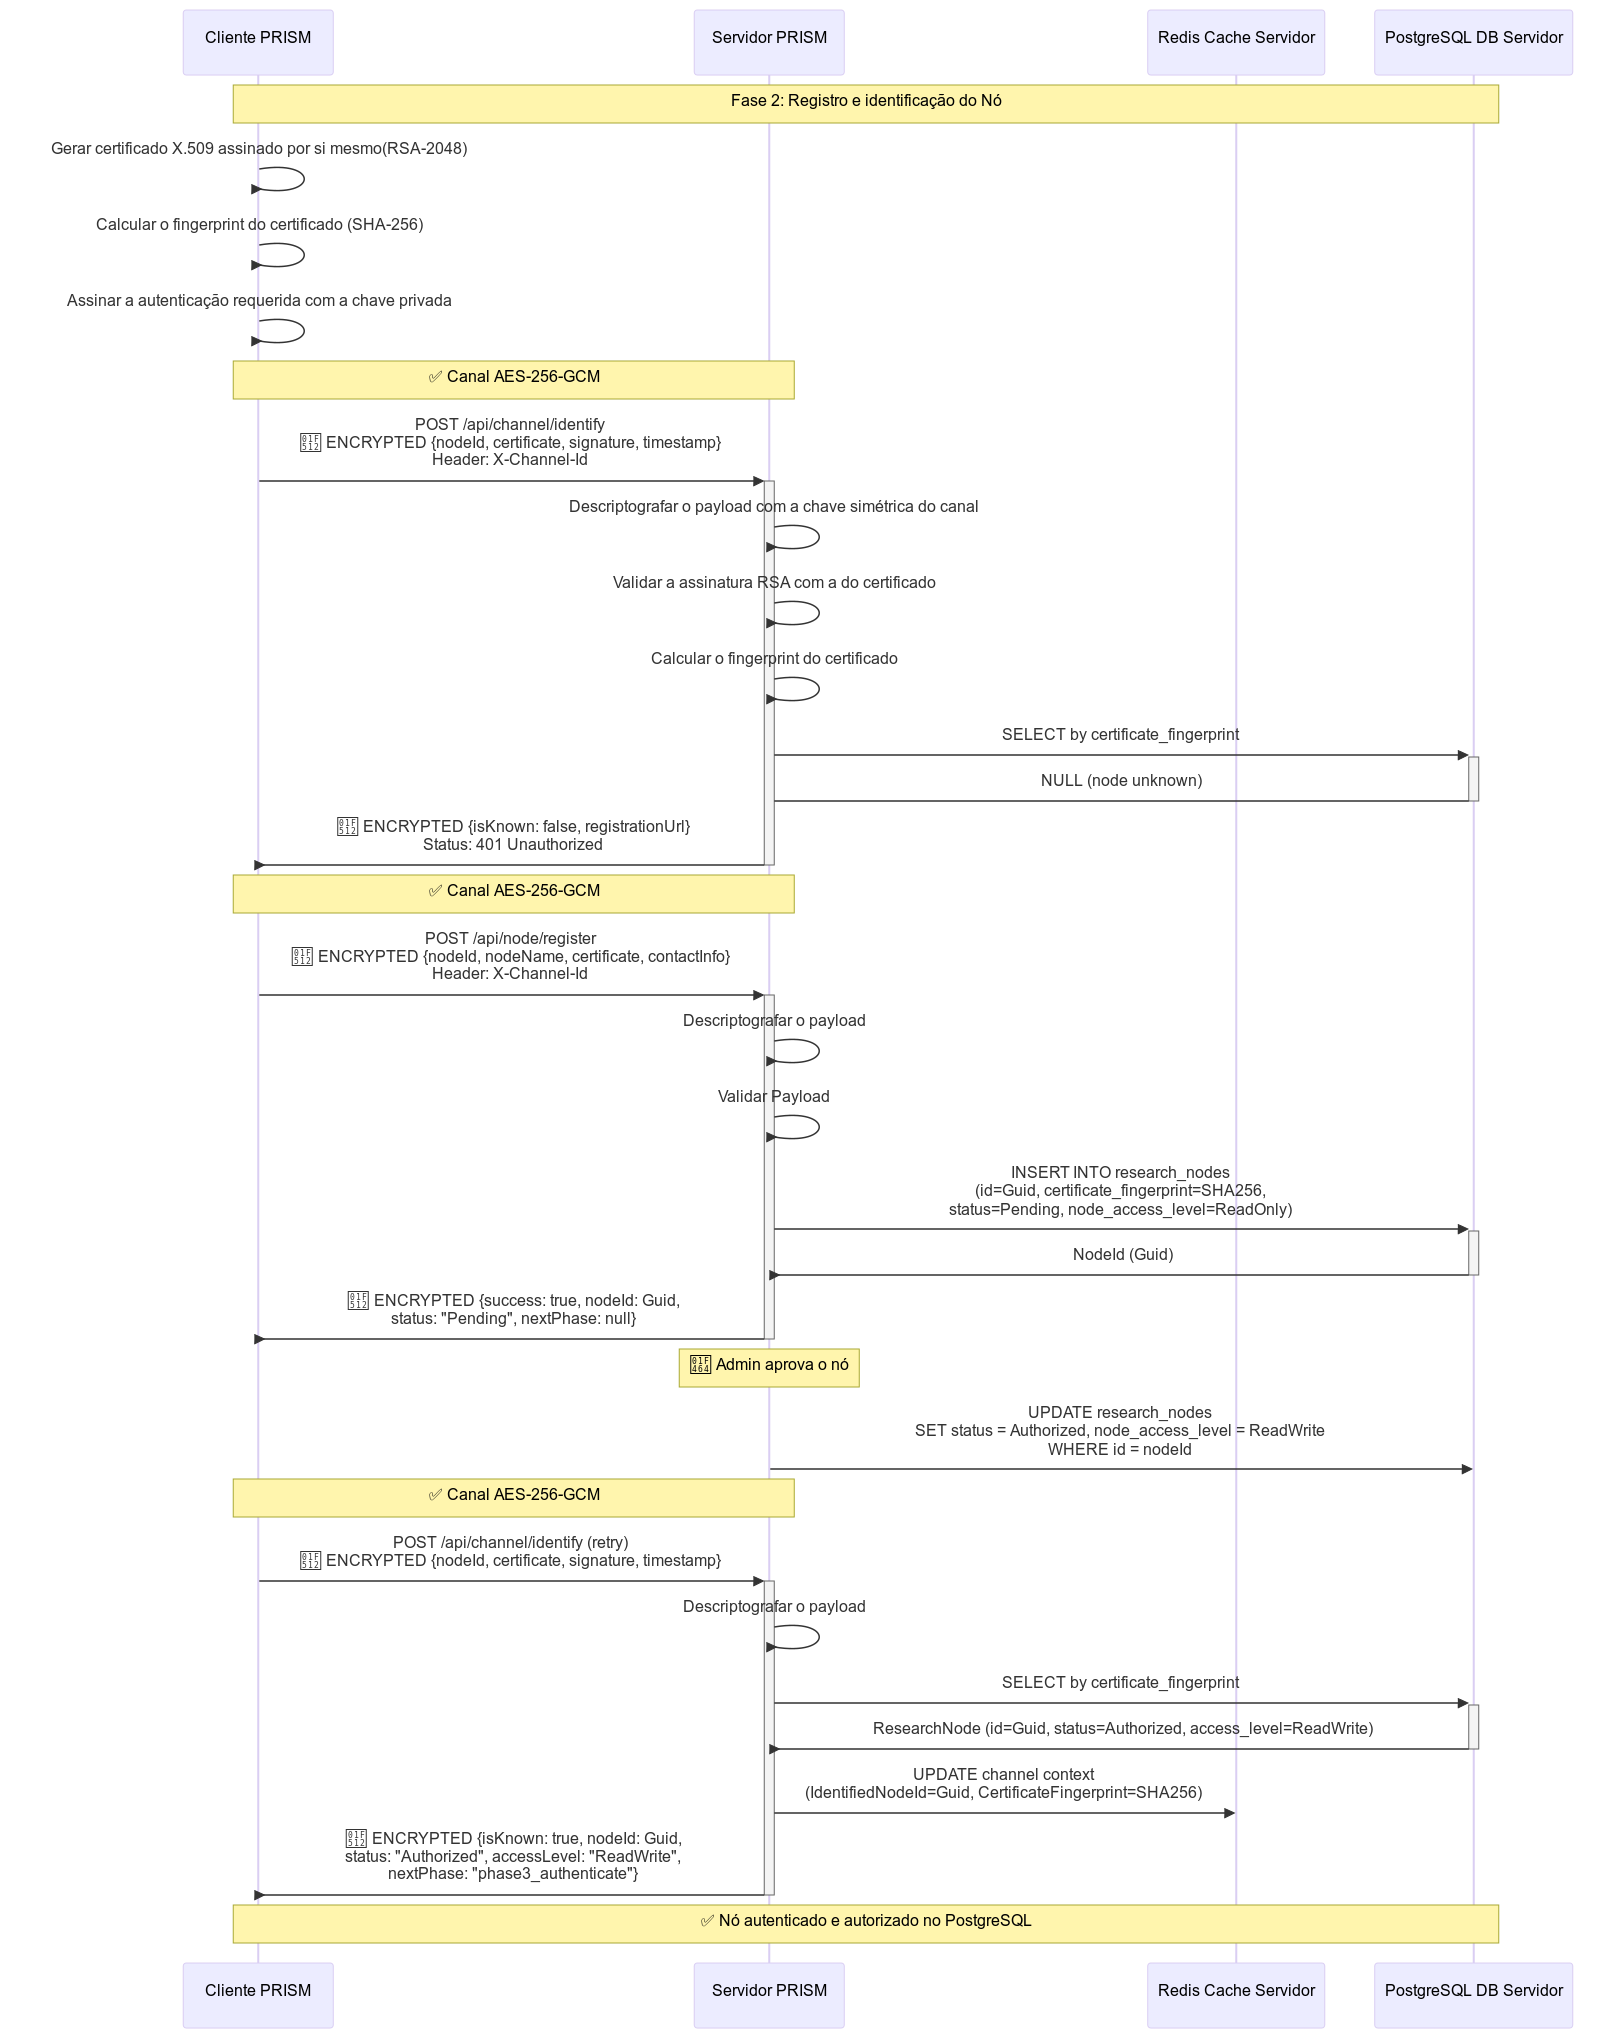
\includegraphics[scale=0.3]{figuras/Desenvolvimento/auth/fase-2.png}%% Dimensões e localização
\fonte{}%% Fonte
\end{figure}

\begin{figure}[htpb]%% Ambiente figure
\captionsetup{width=0.43\textwidth}
\caption{Autenticação mútua por Desafio-Resposta}%% Legenda
\label{fig:auth-fase-3}%% Rótulo
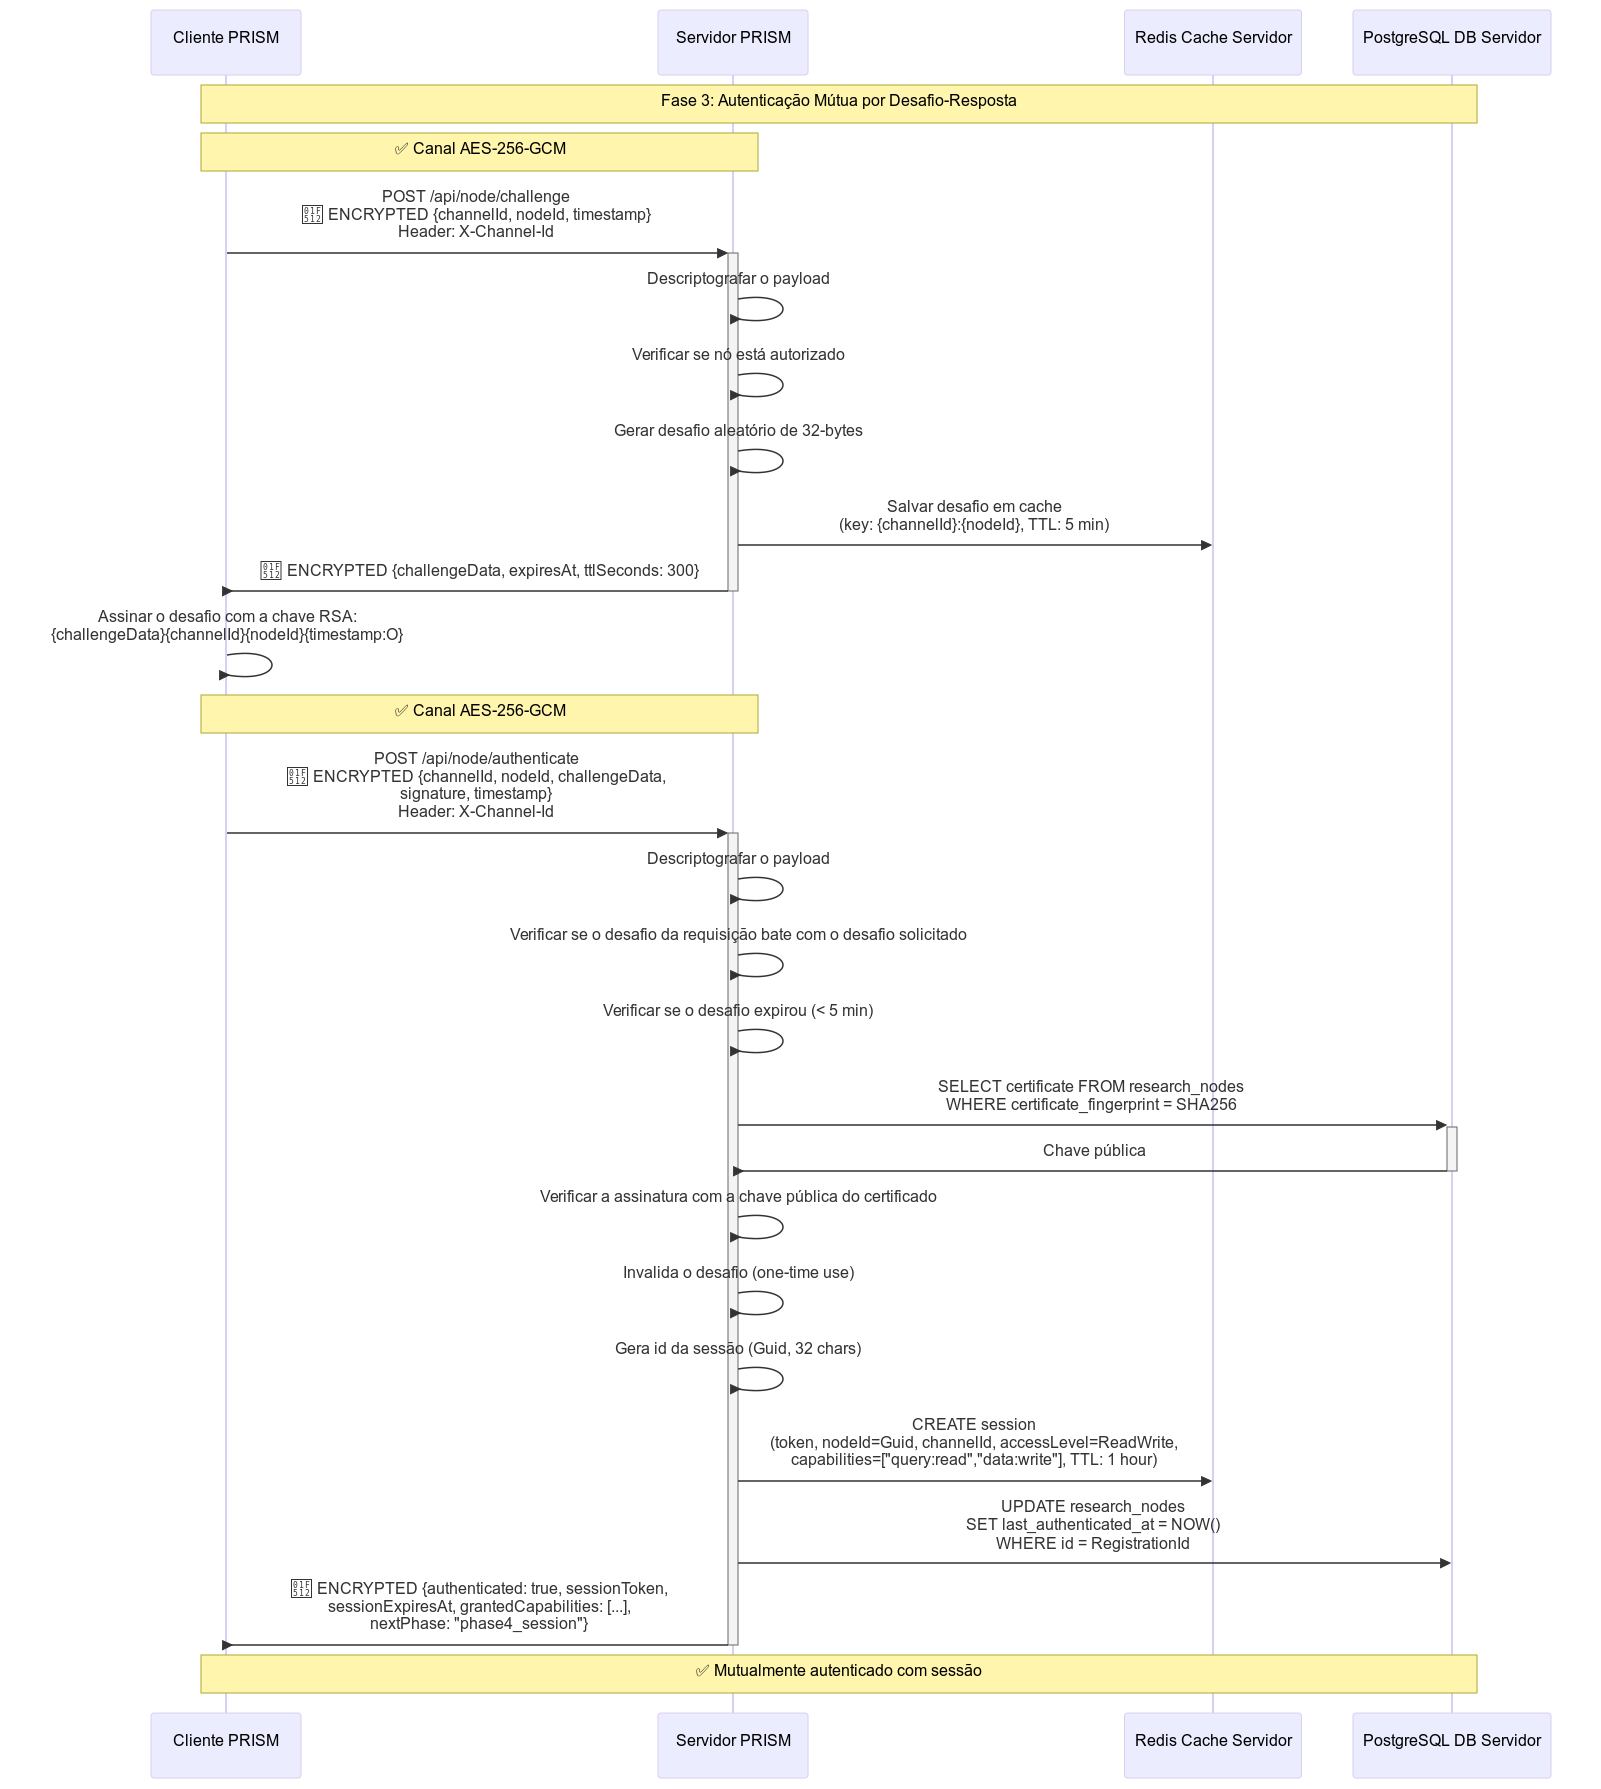
\includegraphics[scale=0.30]{figuras/Desenvolvimento/auth/fase-3.png}%% Dimensões e localização
\fonte{}%% Fonte
\end{figure}

\newpage

A nível de usuário, uma vez a aplicação cliente tenha criado uma uma sessão aberta com o servidor, o usuário da aplicação precisa se autenticar para adicionar e modificar dados presentes no NPI, além de alterar configurações de conexões com outros nós e solicitar

\subsection{Troca de dados}



\newpage
\section{Interoperable Research Interface System - IRIS}\label{sec:desenvolvimentoIRIS}

falar sobre as aplicações bases que serão adicionadas ao nó(Gestão de Acessos, Gestão de pacientes e outras funcionalidades para garantir a facil reusabilidade do projeto

\section{IRIS - Mobile}\label{sec:desenvolvimentoIRISMobile}
\section{Adaptação do NeuroEstimulator}\label{sec:adaptacaoNeuroEstimulator}


O projeto exemplo usado é o NeuroEstimulator, um sistema funcional que 
Explicar sobe o antigo projeto e apontar as modificações que foram necessárias para que se adaptasse as funcionalidades do projeto e exemplificar como integrar com hardware e projetos existente

- Adaptei o código para rodar na taxa fixa de 860hz reduzido para 215hz por média devido a uma limitação do ADC 



Apresenta as funcionalidades e o uso de recursos tecnológicos do sistema por meio de suas telas, enfatizando a interação com o sistema. A apresentação do sistema é feita sob a forma de texto, com telas e definição de padrões que forem relevantes ao contexto do trabalho. As telas são tratadas como figuras, cópias (print screen) de relatórios ou consultas também são figuras.

A \autoref{fig:cadastroPaciente} exibe a tela de acesso ao Cadastro de Pacientes.

\begin{figure}[htpb]%% Ambiente figure
\captionsetup{width=0.43\textwidth}
\caption{Tela de acesso ao Cadastro de Pacientes.}%% Legenda
\label{fig:cadastroPaciente}%% Rótulo

\includegraphics[scale=0.8]{cadastro-paciente}%% Dimensões e localização
\fonte{}%% Fonte
\end{figure}


Um exemplo de listagem de código fonte pode ser observado na \autoref{codigo:classeFoo}, que representa a classe Aluno.

\begin{sourcecode}[htb]
\caption{\label{codigo:classeFoo}Classe Aluno}
\begin{lstlisting}[frame=single, language=Java]
@Entity
public class Foo {
 
    @Id
    @GeneratedValue(strategy = GenerationType.IDENTITY)
    private Long id;
 
    private String nome;
    
    private Integer ra;
     
    // constructor, getters and setters
}
\end{lstlisting}
\fonte{}
\end{sourcecode}
